\documentclass{article}
\usepackage[utf8]{inputenc}
\usepackage{graphicx}
\usepackage{tabu}
\usepackage[spanish]{babel}

\begin{document}
\begin{figure}[t!]

\includegraphics[scale=0.3]{logo_udp.PNG}
\label{fig:udplogo}
\end{figure}



\title{\textbf{{Laboratorio 6 \\ Enrutamiento\vspace{10cm}}}}
\author{\hspace{8cm} Vicente Henriquez \\ \hspace{8cm} Franco Montenegro}
\date{\hspace{8cm} 05/11/2017}



\maketitle
\newpage
\tableofcontents
\newpage
\section{Introducción\vspace{0.5cm}}
En este laboratorio se aprenderá a hacer enrutamiento, así mismo se aprenderá a configurar y analizar la importancia de dos de los protocolos de ruteo, uno se denomina EIGRP y el otro OSPF, se usará packet tracer para el configuramiento de ruteo.
\newpage
\section{Desarrollo\vspace{0.5cm}}
\subsection{Actividad\vspace{0.3cm}}
El objetivo de nuestra actividad es entender y aprender a configurar dos protocolos de ruteo: EIGRP y OSPF.
Para la primera parte de la actividad se procederá a configurar la topología de la Figura \ref{fig:topo} con el protocolo EIGRP:

\begin{figure}[h!]
\centering
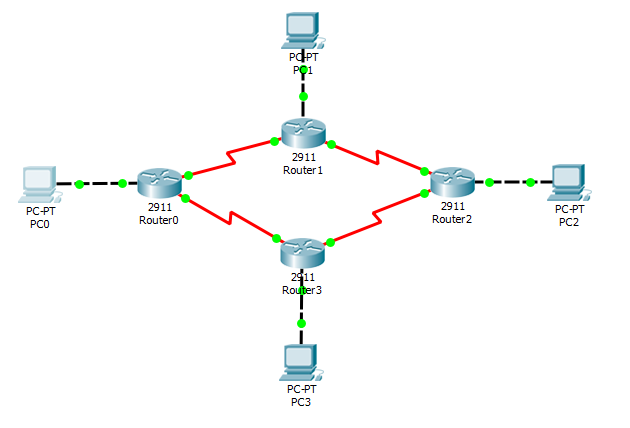
\includegraphics[scale=0.6]{Top.png}
\caption{Topología}
\label{fig:topo}
\end{figure}

Para las conexiones entre routers se usaran los siguientes comandos:

\begin{figure}[h!]
\centering
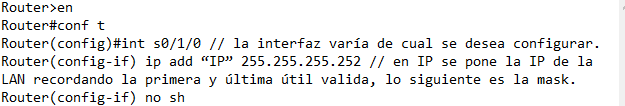
\includegraphics[scale=0.65]{EntreR.png}
\caption{Comandos entre Routers}
\label{fig:com1}
\end{figure}

Al igual que en la Figura \ref{fig:ejem1} ,se utilizarán los comandos anteriormente mencionados en todas las conexiones entre routers de la topología. Como buena práctica es recomendable anotar las sX/X/X e Ips que se utilicen.

\newpage

\begin{figure}[h!]
\centering
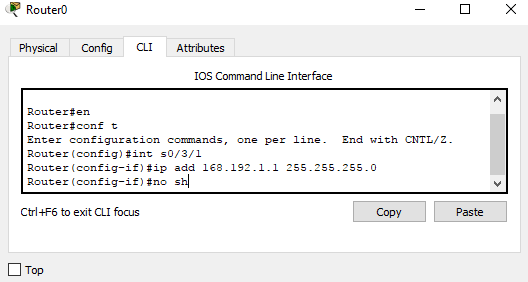
\includegraphics[scale=0.65]{Ej1.png}
\caption{Ejemplo - Comandos entre Routers}
\label{fig:ejem1}
\end{figure}

Luego, para las conexiones entre el routers y sus respectivas LANs se utilizarán los siguientes comandos:

\begin{figure}[h!]
\centering
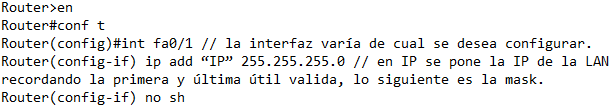
\includegraphics[scale=0.65]{RouLan.png}
\caption{Comandos entre Routers y LANs}
\label{fig:com2}
\end{figure}

Ejemplo de los comandos mencionados siendo utilizados en nuestra topología:

\begin{figure}[h!]
\centering
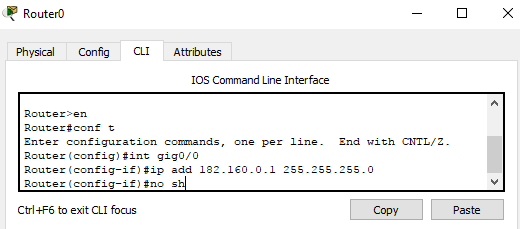
\includegraphics[scale=0.65]{Ej2.png}
\caption{Ejemplo - Comandos entre Routers y LANs}
\label{fig:ejem2}
\end{figure}

\newpage

Para la segunda parte de la actividad, configuraremos los protocolos de ruteo para EIGRP, presentes en la siguiente figura:

\begin{figure}[h!]
\centering
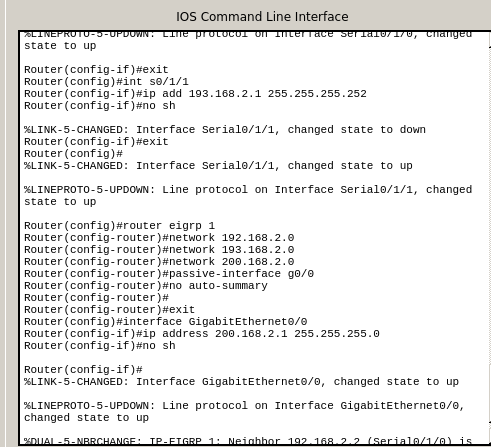
\includegraphics[scale=0.65]{Actpart2.png}
\caption{Comandos para EIGRP}
\label{fig:com3}
\end{figure}

Quedando así la configuración de los routers (en la Figura \ref{fig:ej3} sólo se muestra uno como ejemplo para todos):

\begin{figure}[h!]
\centering
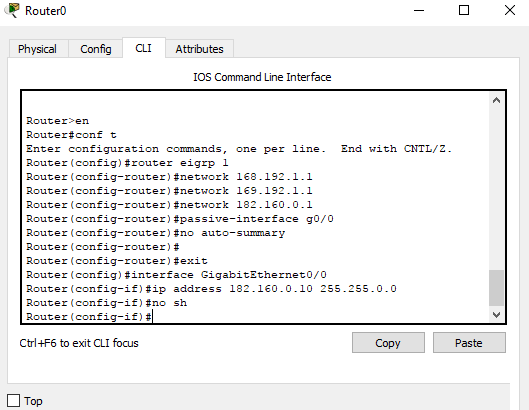
\includegraphics[width=11cm, height=6.5cm]{Ej3.png}
\caption{Ejemplo - Comandos para EIGRP}
\label{fig:ej3}
\end{figure}

\newpage
\subsection{Preguntas\vspace{0.3cm}}
\begin{enumerate}
\item ¿Cuál es la diferencia entre los algoritmos de Dijkstra y Bellman Ford?\\
\newline La diferencia entre los algoritmos de Dijkstra y bellman Ford es que el algoritmo de bellman Ford si utiliza los pesos negativos de alguna de las aristas para generar el camino más corto en un grafo dirigido, a diferencia del algoritmo de Dijkstra que busca el camino más fácil, pero con la excepción de que la arista no puede tener peso negativo.

\item Mencione dos protocolos de ruteo de cada algoritmo (Dijkstra y Bellman Ford)\\
\newline Del algoritmo de Dijkstra dos protocolos son OSPF e IS-IS, por otro lado, del algoritmo de Bellman Ford se encuentran RIP (versión 1 y 2) e IGRP.

\item ¿Qué es más eficiente: IGRP u OSPF? ¿Por qué?\\
\newline El uso de uno de estos protocolos depende de diferentes factores, si se presenta una red de mediano o gran tamaño lo mejor sería utilizar OSPF ya que es abierta y permite cualquier equipo, imaginar gestionar rutas de una gran cantidad de equipos, con la desventaja de la difícil configuración, para redes más pequeñas es mejor IGRP que tiene una configuración más fácil.

\item ¿En qué caso usaría vector distancia y en cuál estado de enlace?\\
\newline Cuando la red es simple y plana sin diseño jerárquico especial es mejor utilizar vector distancia, si la red tiene un diseño jerárquico y es de gran tamaño es conveniente utilizar estado de enlace.

\item ¿Qué algoritmo tiene menor tiempo de convergencia si se agrega un nuevo equipo a la red?\\
\newline Si se agregase un nuevo equipo a la red el algoritmo que tiene menor tiempo de convergencia es estado de enlace ya que los cambios en la red son inmediatamente introducidos en el dominio.


\end{enumerate}

\newpage
\section{Conclusión \vspace{0.5cm}}
En este laboratorio se pudo comprender la importancia de los protocolos de ruteo según los diferentes algoritmos presentados y cómo influyen en la red, según el tipo de red que tengamos.

\end{document}
